\section{Event Representation}\label{sec:model}

We introduce our model and the methodology for applying it to messages that
describe events in social media.

% We introduce a scalable high-level news event representation from microblog data, leveraging
% social media features such as redundancy. Specifically, we define our
% representation and some possible applications.
% The key idea of our representation is to leverage redundancy, common information
% across messages, to reduce the amount of resulting documents while increasing
% the effectiveness of the corpus.
% %, and to be able to easily identify different aspects of an event. 
% For that, we use the shared URLs as clues to aggregate messages into a single
% {\em document}. Our assumption is that the content of the messages that mention
% the same URLs refer to the same aspect of an event. For example, if an URL
% points to an image of a destroyed building (e.g., in the context of an
% earthquake), then it is highly likely that the text of all the messages
% containing that URL will refer to the building and not to a different topic. We
% say that the text in those messages is a {\em surrogate} of the content in the
% URL. This allows us to annotate multimedia content using social media
% information. At the same time, we can reduce the amount of messages by
% aggregating them into a single document, resulting in a more scalable
% representation. 
% We also incorporate other social interactions, such as forward or reply
% messages. For example, in Twitter they are called {\em retweets} and replies,
% respectively. The assumption is similar, and the action of forwarding or
% replying a message can be seen as sharing the URL of the message being
% forwarded or replied, as well.


% Idea: presentar el modelo con la suposicion de que las URLs que tenemos son las
% buenas, es decir, identifican "bien" un topico del evento, a diferencia de las
% urls que no (las que tienen mucho grado en el grafo de coocurrencia). Luego, en
% la metodologia, mostrar una forma de identificar las urls buenas usando el graof
% de coocurrencia.
% tres tipos de urls: "especificas" (topic-specific), generales e irrelevantes

%\paragraph{\bf{Representation definition}}

Our model is based on the assumption that {\em most of the social media posts
that discuss a specific event and contain a URL, are messages that cover a
particular portion or sub-topic of the event}.
%
For example, in the case of an earthquake, tweets that refer to damages to
buildings may share a URL to an external news report; similarly, a tweet that
discusses the magnitude of the event may link to the official seismological
report.
%
We define an event as a tuple $\mathcal{E} = (M, U)$, where $M$ is the set of
messages that discuss a real-world occurrence, and $U$ is
the set of {\em topic-specific} URLs that are mentioned or shared by messages in
$M$. 
%
We denote the URLs $U$ as {\em topic-specific}, assuming that each URL in $U$
identifies only one of the different topics within the real-world event.
%
Our representation is a graph $\mathcal{G} = (V, E)$, where $V \subseteq M \cup
U$ is the set of nodes, comprised of {\em messages} and {\em URLs}, and there is
an edge $(i, j) \in E$ if at least one of the following conditions hold: (1)
$m=i$ is a message and $u=j$ is a URL and $m$ shares $u$, (2) $m_1=i$ and
$m_2=j$ are messages and $m_1$ re-shares $m_2$, or (3) $m_1=i$ and $m_2=j$ are
messages and $m_1$ replies to $m_2$ (see an example in
Figure~\ref{fig:model-example}).
%
Finally, a {\em document} is a connected component of $\mathcal{G}$.
%
In this case, a document is defined as a collection of messages that discuss
only one aspect of the event.

%%

The assumption of $U$ to be a set of topic-specific URLs may not hold in all
cases, for example, for URLs that address general aspects of an event (e.g., a
summary report of an entire event), or that are generic (e.g., refer to a online
news website's root URL), or irrelevant to the event (e.g., spam, or unrelated
information).
%
We deal with these cases in our methodology for generating event models,
presented below.
% In other cases, a message could share more than one URL, and the two of them can
% be complementary, for example, sharing a news report along with a relevant image
% or video.
%
In that sense, our model and methodology focus on identifying URLs that are
specific to one aspect of an event, and use those URLs to aggregate similar
messages.
%
Our goal is to represent underlying sub-topics of an event by just using shared
URLs. 


%%

%\bp{creo que lo anterior esta incompleto y algo confuso: Falta decir que en realidad una componente conexa es un documento (al final esta es la representacion). Tambien hay que decir que en realidad una componente se entiende como elementos que hablan de lo mismo y por eso se modelan como un unico documento. El resto de identificar urls problematicas esta bien que quede en la metodologia.}

\begin{figure}[t]
  \centering
  \resizebox {0.6\columnwidth} {!} {
    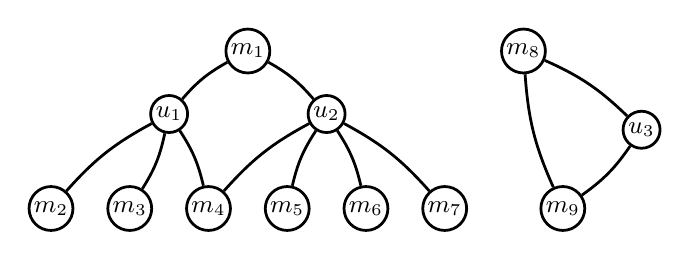
\begin{tikzpicture}[
    every edge/.style={draw, line width=1pt, align=left, sloped}
    ]
  
    \node[draw, circle, inner sep = 1pt, line width=1pt] (m1) at (0, 0) {\small $m_1$};
    \node[draw, circle, inner sep = 1pt, line width=1pt] (u1) at (-1, -0.8) {\small $u_1$};
    \node[draw, circle, inner sep = 1pt, line width=1pt] (u2) at (1, -0.8) {\small $u_2$};
    
    \node[draw, circle, inner sep = 1pt, line width=1pt] (m2) at (-2.5, -2) {\small $m_2$};
    \node[draw, circle, inner sep = 1pt, line width=1pt] (m3) at (-1.5, -2) {\small $m_3$};
    \node[draw, circle, inner sep = 1pt, line width=1pt] (m4) at (-0.5, -2) {\small $m_4$};

    \node[draw, circle, inner sep = 1pt, line width=1pt] (m5) at (0.5, -2) {\small $m_5$};
    \node[draw, circle, inner sep = 1pt, line width=1pt] (m6) at (1.5, -2) {\small $m_6$};
    \node[draw, circle, inner sep = 1pt, line width=1pt] (m7) at (2.5, -2) {\small $m_7$};
  
    \path [-] (m1) edge[bend right=10] node[below=1pt] {} (u1);
    \path [-] (m1) edge[bend left=10] node[below=1pt] {} (u2);

    \path [-] (m2) edge[bend left=10] node[below=1pt] {} (u1);
    \path [-] (m3) edge[bend right=10] node[below=1pt] {} (u1);
    \path [-] (m4) edge[bend right=10] node[below=1pt] {} (u1);
    \path [-] (m4) edge[bend left=10] node[below=1pt] {} (u2);
    
    \path [-] (m5) edge[bend left=10] node[below=1pt] {} (u2);
    \path [-] (m6) edge[bend right=10] node[below=1pt] {} (u2);
    \path [-] (m7) edge[bend right=10] node[below=1pt] {} (u2);


    \node[draw, circle, inner sep = 1pt, line width=1pt] (m8) at (3.5, 0) {\small $m_8$};
    \node[draw, circle, inner sep = 1pt, line width=1pt] (u3) at (5, -1) {\small $u_3$};
    \node[draw, circle, inner sep = 1pt, line width=1pt] (m9) at (4, -2) {\small $m_9$};

    \path [-] (m8) edge[bend right=10] node[below=1pt] {} (m9);
    \path [-] (m9) edge[bend right=10] node[below=1pt] {} (u3);
    \path [-] (m8) edge[bend left=10] node[above=1pt] {} (u3);

  \end{tikzpicture}
  }
  \caption[Example representation of messages.]{
    Example representation of messages. On the left side, 
    messages $m_1$ and $m_4$ share URLs $u_1$ and $u_2$, while $m_2$ only shares $u_1$.
    On the right side, $m_8$ and $m_9$ share or reply one to another, and also share URL $u_3$. 
    Each connected component is a {\em document}.
  }
  \label{fig:model-example}

\end{figure}

% \begin{figure}
%   \centering
%     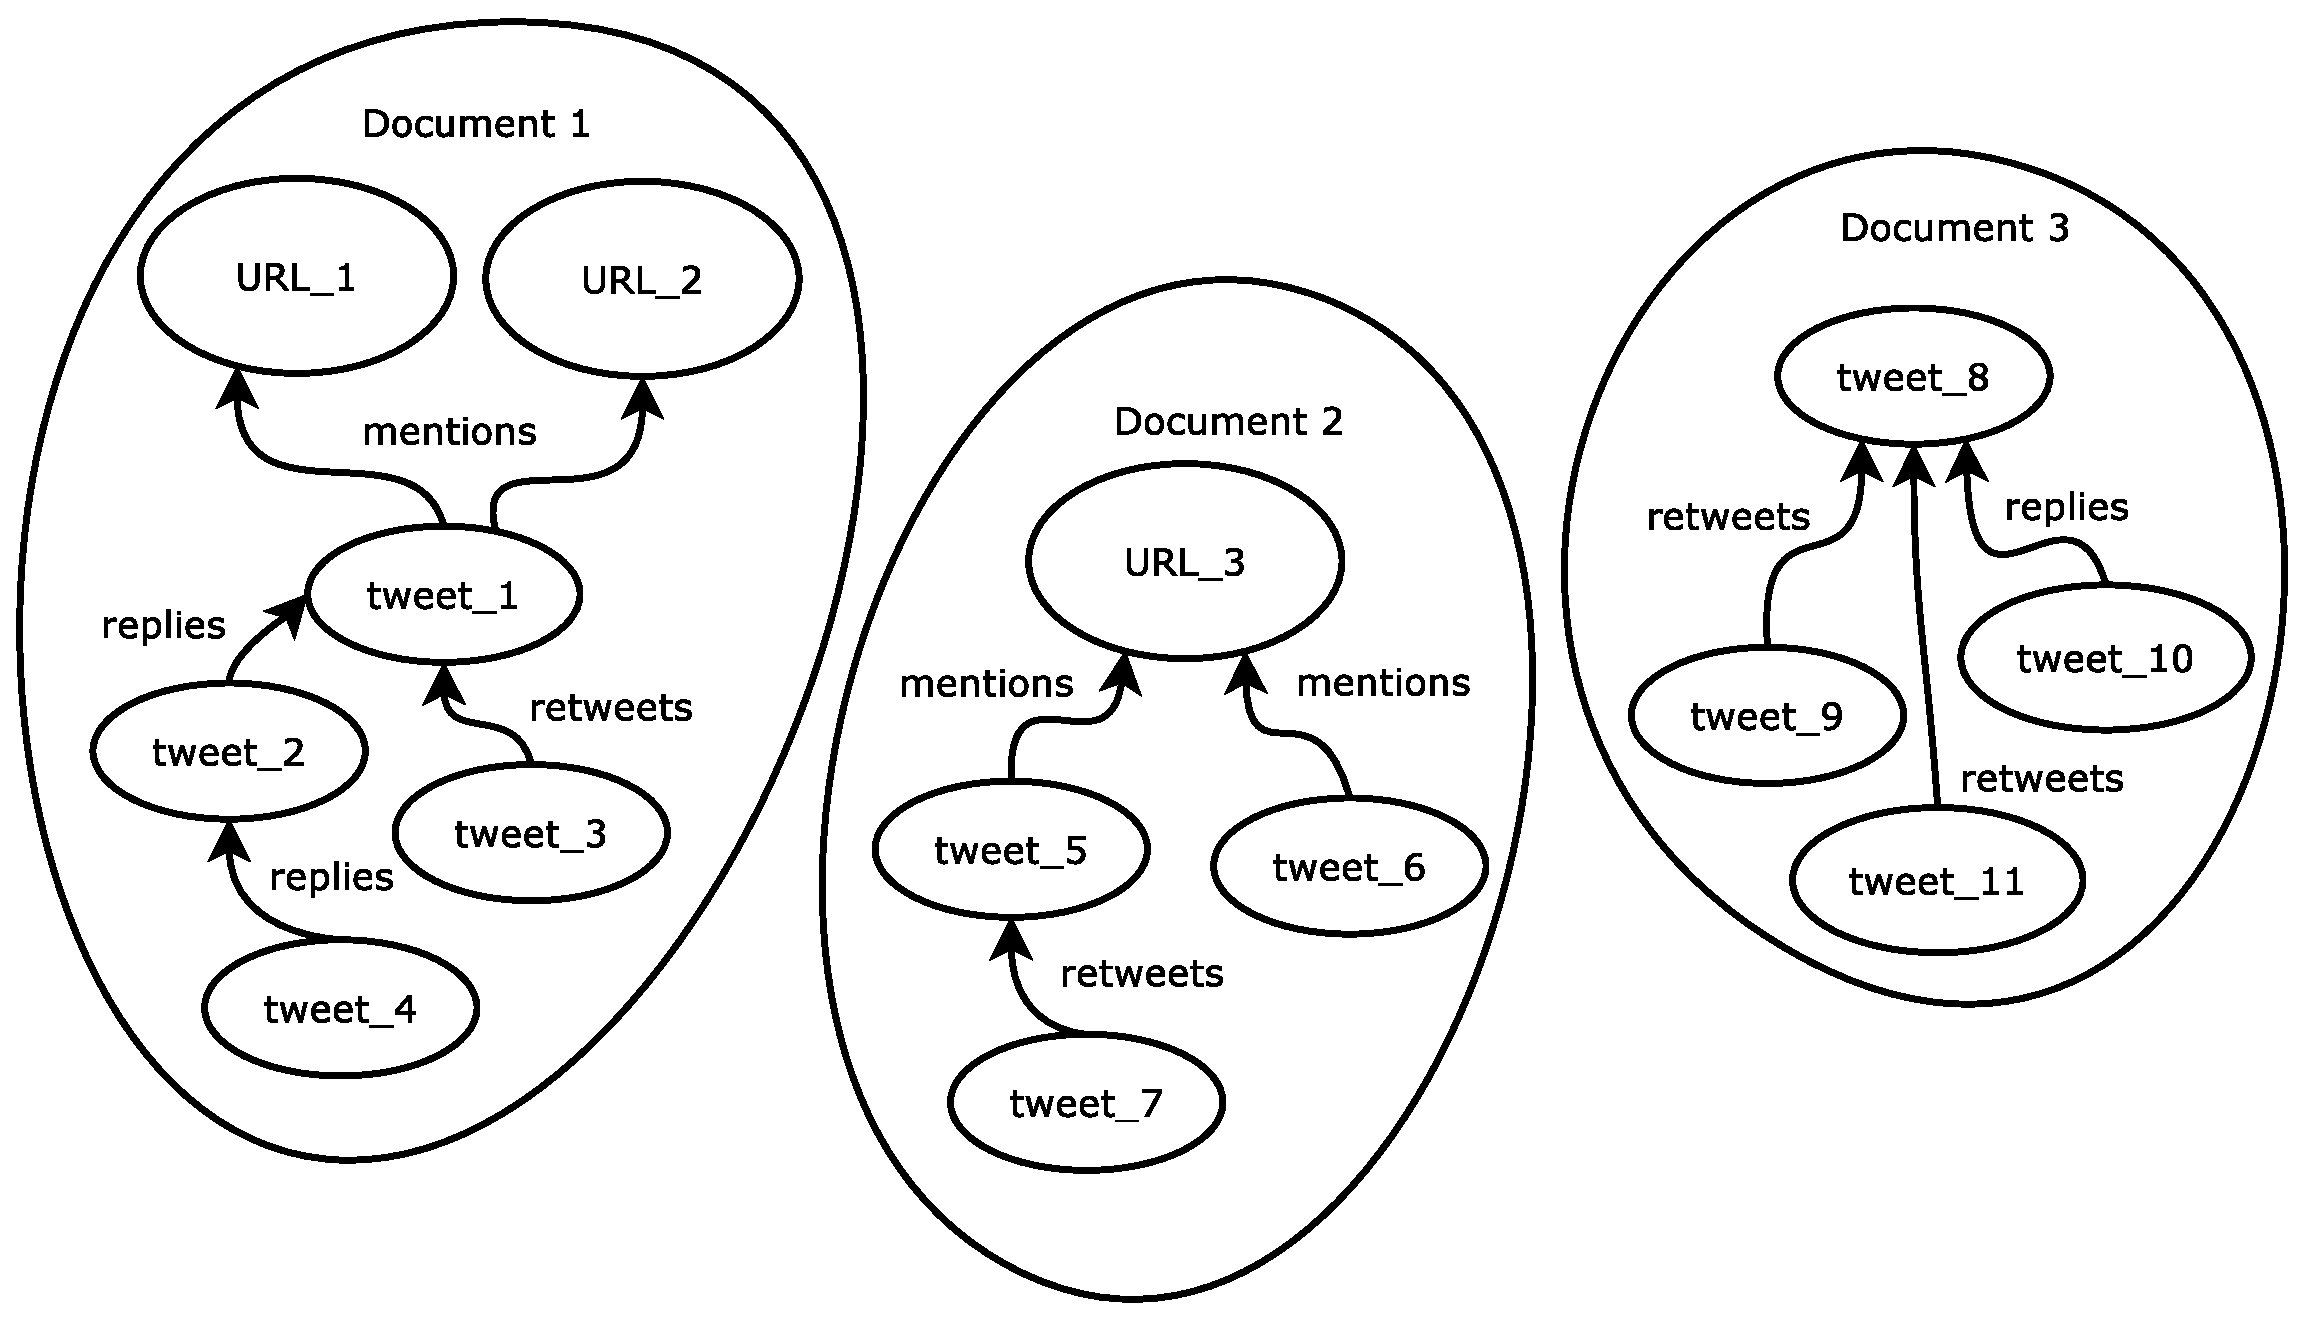
\includegraphics[width=0.4\textwidth]{fig/docs.eps}
%   \caption{Conceptual example of documents. A document is a set of messages that share or reply each other, and the messages that share the same URL. In order to have a representative element for each document, only documents with URL can be considered, and documents with multiple URLs can be duplicated, while each document has a different URL.
%   }\label{fig:model}
% \end{figure}

% Consider Twitter as an example. A document $d$ is a set of URLs, plus the tweets
% that mention those URLs, plus the tweets that retweet or reply any of the
% tweets in $d$. Note that if there are more than one URL, then there should be
% at least one tweet that mention all those URLs, or there is a path of replies
% or retweets between the tweets that mention those URLs individually.
% Figure~\ref{fig:model} shows an example of a few documents.

% \begin{algorithm}
% \caption{Model generation}\label{algo:gen}

% \SetAlgoLined
% \KwData{Messages $T$, URLs $U$ mentioned in messages in $T$}
% \KwResult{Documents $D = \{d_1, d_2, \ldots, d_N\}$, with $d_i\subseteq T\cup U$, for $i\in \{1, \ldots N\}$}
%  $Pairs \leftarrow \emptyset$\;
%  \For{$t \in T$}{
%   \For{$u \in U$ that is mentioned by $t$} {
%     $Pairs \leftarrow Pairs \cup \{(t, u)\}$\;
%   }
%   \If{$\exists t' \in T$ such that $t$ replies to or forwards $t'$}{
%    $Pairs \leftarrow Pairs \cup \{(t, t')\}$\;
%   }
%  }
%  \For{$u \in U$} {
%   \em{UnionFind}.makeSet$(u)$\;
%  }
%  \For{$(p, q) \in Pairs$} {
%   \em{UnionFind}.union$(p, q)$\;
%  }
%  $D \leftarrow UnionFind.sets()$\;
% \end{algorithm}
% \vspace{-0.5cm}

%%%%%%%%%%%%%%%%%%%%%%%%%%%%%%%%%%%%%%%%%%%%%%%%%%%%%%%%%%%%%%%%%%%%%%%%
%%%%%%%%%%%%%%%%%%%%%%%%%%%%%%%%%%%%%%%%%%%%%%%%%%%%%%%%%%%%%%%%%%%%%%%%
%%%%%%%%%%%%%%%%%%%%%%%%%%%%%%%%%%%%%%%%%%%%%%%%%%%%%%%%%%%%%%%%%%%%%%%%
%%%%%%%%%%%%%%%%%%%%%%%%%%%%%%%%%%%%%%%%%%%%%%%%%%%%%%%%%%%%%%%%%%%%%%%%


%\paragraph{\bf{Generation methodology}}\label{sec:methodology}

\subsection*{Methodology for representing events}

Given a set of event-related social media messages, we propose the following
methodology for representation generation:
  
{\bf Filter out generic URLs:} 
%
We call generic URLs (too general with respect to the event) as those that
co-occur with multiple different other URLs across many messages.
%
A URL co-occur with another one URL if they both are shared by the same message.
%
Highly connected URLs are assumed to not contribute information to specific topics: 
links that are very generic (e.g., {\tt cnn.com}) or very general to the event 
(e.g., general reports). 
%
All of the messages mentioning these URLs would fall into the same component,
regardless of their differences in content. 
%
We removed URLs that co-occurred with three or more different URLs across
messages.
%
This threshold yielded the best results in our case studies.


{\bf Representation generation:} 
%
The generation step consists of grouping messages that end up in the same
component, as described in the previous section.
%
For that, a straightforward method is to compute all pairs of messages and pairs
of URLs and messages that fulfill the conditions stated in the representation
definition and then find connected components using a union-find algorithm.
%
The URLs are the non-generic ones identified in the previous step, as an
approximation to the topic-specific URLs.


{\bf Vector representation of documents:} 
%
Finally, we aggregate messages into documents in order to produce a vector
representation, using neural network-based word embeddings.
%
This procedure generates dense document representations.
%
To aggregate messages, we simple compute a vector representation of each word in every message and 
then aggregate all the vectors (for example, using the mean or the sum of all vectors).




% Our goal is to propose a methodology for generating automatic summaries from
% news events on Twitter, exploiting both the multimedia content and the
% importance that users give to certain topics. For that, we learned a
% representation of the URLs shared from event-related tweets (URLs pointing to
% images, videos, other tweets, or other Web pages in general), using the text in
% the tweets that surround those URLs, borrowing the idea of anchor texts in query
% log mining. We used this representation to group the URLs into clusters and then
% used the social features of each tweet in order to rank the URLs and the
% clusters, based on the level of activity that users had on each of those. This
% allowed us to sort the different aspects of an event based on the importance
% that users give to them.



% \subsection{Definitions}

% \paragraph{Tweet} A {em tweet} can be seen as a struct with the following fields:

% \begin{itemize} \item {\em text}: the textual content of the tweet. \item {\em creation\_date}: a
% timestamp when the tweet was published. \item {\em no\_retweets}: the amount of times that tweet was
% shared or       forwarded by other users. \item {\em no\_likes}: the amount of times users ``liked''
% the tweet. \item {\em user}: an identifier of the user who published the tweet. \end{itemize}


% \paragraph{Summary} Given a set of tweets $E = \{t_1, t_2, \ldots, t_N\}$, called an {\em   event},
% we want to select a subset $S \subseteq E$ of tweets, called   a {\em summary}. The summary must
% fulfill the following criteria:

% \begin{itemize}      
% \item {\bf Topical coverage}: the tweets in $S$ must cover the same topics as
% $E$.   \item {\bf Redundancy}: the content of tweets in $S$ must not be redundant with each other.

% \item {\bf Importance}: the tweets in $S$ must be the top $|S|$, with respect to $E$, according to a
% pre-defined ranking function, considering into account the previous two criteria. For example, if
% two tweets have the same value according to the ranking, but     the two of them are equal in terms
% of content, then only one of them should be in $S$.   

% \item {\bf Human-manageable size}: the size of
% $S$ must be of much less size than $E$, only if $E$ is large. {\bf (TODO: define what is ``large''
% and how less is ``less.'')} \end{itemize}

% \paragraph{Replies and retweets} We denote by $\mathit{URL}(t) = \{u_1, u_2, \ldots, u_m\}$ the URLs
% shared by the tweet $t$. $\mathit{URL}(t)$ is empty if $t$ does not share any URL.

% We also denote by $\mathit{replies}(t)$ the set of all tweets $t'$ such that $t'$ is a {\em reply}
% of $t$, or $t'$ is a reply of another tweet in $\mathit{replies}(t)$. The same applies to
% $\mathit{retweets}(t)$, but by considering {\em retweets} instead of replies.

% \paragraph{Document} We now define a {\em document} $d_u$ as a set of tweets, such that those tweets
% share the same URL $u$, plus their replies and retweets, that is,



% Note that a tweet $t$ can be a member of different documents, if $t$ shares more than one URL.


% \subsection{Methodology}

% We make use of the context of multiple tweets in order to arrange them into topically similar
% groups. When a tweet shares an URL $u$, the content of the tweet can be seen as a description (or
% {\em anchor text}) or a comment on the content of $u$. This also applies when a tweet is a {\em
% reply} of another tweet: those two tweets (the reply and the replied) are topically similar, because
% both of them refers to the same subject of discussion. We use this context to group tweets into
% documents.

% Given an event $E$, let $U$ be the set of all the URLs shared across tweets in $E$. The documents
% induced by $U$ are all the subsets of tweets that share at least one URL, $D = \{d_u\ :\ u \in U\}$.
% Our goal is to select representative tweets to create $S$, by using $D$ as a proxy by grouping
% similar tweets into documents.

% One main task is to compare documents. Two documents whose content is topically similar should be
% similar according to the features of its constituents. Note that the documents may have very
% different sizes, and it is possible that two different documents are topically similar. This makes
% comparing documents a difficult task.

% By comparing documents, our goal is to discover sub-topics inside $E$, in order to achieve coverage
% in the resulting summary. Possible implementations for sub-topic identification are clustering (e.g.
% K-Means, K-Medoids, hierarchical, or online/incremental), or process an induced graph from the
% documents (e.g. community detection, connected components, or centrality measures). Another
% alternative, which does not require computing a similarity measure between documents, is the use of
% topic modelling (LDA or Dynamic Topic Models if the time dimension is considered).


% \paragraph{Similarity between documents}

% There are two alternatives when computing similarity between documents:

% \begin{enumerate} \item {\em Consider all the elements of a document as a single element.} For
% example, compute a vector space model (e.g. tf-idf) over the concatenation of tweets in a document
% and then compare the representations using standard cosine similarity. A problem with this approach
% is that diverse content inside a document can be shadowed by the most popular content inside a
% document. Or, on the other hand, if there is a lot of diverse content, then the focus of the
% document can be inaccurate, compared by a smaller, focused document.

% \item {\em Consider each element of a document as a single element.} For example, compare individual
% pairs of tweets of different documents, and then compute an average of similarities to assess the
% similarity of the two documents. This could share a similar problem with the other alternative, as
% diverse content may diffuse the main focus of a document (or be shadowed by the popular content).
% Another alternative is to derive high similarity between unequally-sized documents if {\em some} of
% the tweets in the larger document are {\em very} similar to the tweets in the smaller one.

% Another problem is the sparsity of vocabulary of tweets, if we compare them one by one. But this can
% be settled by using more information about the tweets (for example, by using a word embedding to
% compute similarity between words). \end{enumerate}

% The second approach may be better adjusted to the specific domain, where certain topics of an event
% are way more popular than the rest.